\documentclass[tikz,border=3pt]{standalone}
\usepackage[utf8]{inputenc}
\usepackage[T1]{fontenc}
\usepackage{lmodern}
\renewcommand{\familydefault}{\sfdefault}
\usepackage{sansmath}\sansmath
\usepackage{chemfig}
\usepackage{pgfplots}\pgfplotsset{compat=1.18,/pgf/number format/use comma,/pgf/number format/1000 sep={.}}
\usetikzlibrary{arrows.meta,calc,positioning,decorations.pathmorphing,patterns}
% paleta del sitio
\definecolor{nar}{HTML}{E8680C}\definecolor{narc}{HTML}{FFB35C}\definecolor{hielo}{HTML}{FFF3E8}
\definecolor{tinta}{HTML}{1D1D1F}\definecolor{gris}{HTML}{6E6E73}\definecolor{lila}{HTML}{7C5CF0}
\definecolor{azul}{HTML}{2F6FD6}\definecolor{menta}{HTML}{17A673}\definecolor{coral}{HTML}{E8342A}
\begin{document}
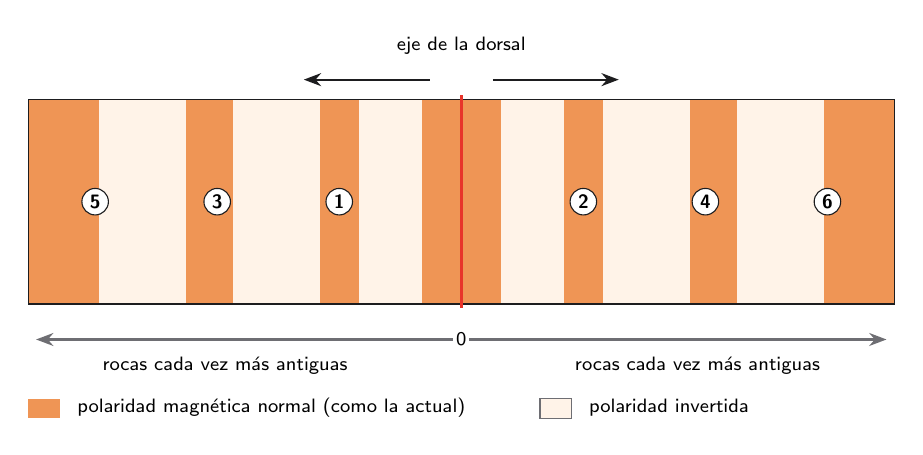
\begin{tikzpicture}[font=\footnotesize,>={Stealth[length=2.2mm]}]
% franjas magneticas simetricas (vista desde arriba)
\def\H{2.6}
\fill[hielo] (-5.5,0) rectangle (5.5,\H);
\foreach \a/\b in {0/0.5,1.3/1.8,2.9/3.5,4.6/5.5} {
  \fill[nar!70] (\a,0) rectangle (\b,\H);
  \fill[nar!70] (-\b,0) rectangle (-\a,\H);
}
\draw[tinta] (-5.5,0) rectangle (5.5,\H);
\draw[coral,very thick] (0,-0.05) -- (0,\H+0.05);
\node[font=\scriptsize,anchor=south] at (0,\H+0.45) {eje de la dorsal};
\draw[->,thick,tinta] (0.4,\H+0.25) -- (2.0,\H+0.25);
\draw[->,thick,tinta] (-0.4,\H+0.25) -- (-2.0,\H+0.25);
% puntos de muestreo
\foreach \n/\x in {1/-1.55,2/1.55,3/-3.1,4/3.1,5/-4.65,6/4.65}
  \node[circle,draw=tinta,fill=white,inner sep=1.2pt,font=\scriptsize\bfseries] at (\x,1.3) {\n};
% eje de edad
\draw[->,thick,gris] (0,-0.45) -- (5.4,-0.45);
\draw[->,thick,gris] (0,-0.45) -- (-5.4,-0.45);
\node[font=\scriptsize,fill=white,inner sep=1pt] at (0,-0.45) {0};
\node[font=\scriptsize,anchor=north] at (3.0,-0.55) {rocas cada vez más antiguas};
\node[font=\scriptsize,anchor=north] at (-3.0,-0.55) {rocas cada vez más antiguas};
% leyenda
\fill[nar!70] (-5.5,-1.45) rectangle (-5.1,-1.2); \node[anchor=west,font=\scriptsize] at (-5.0,-1.32) {polaridad magnética normal (como la actual)};
\fill[hielo] (1.0,-1.45) rectangle (1.4,-1.2); \draw[gris] (1.0,-1.45) rectangle (1.4,-1.2);
\node[anchor=west,font=\scriptsize] at (1.5,-1.32) {polaridad invertida};
\end{tikzpicture}
\end{document}
